\section{Directory Structure}
\todo[inline]{Wollen wir hier alle Unterordner kurz vorstellen und \emph{kurz} erklären,
  was in deren Unterordnern zu finden ist?}
We briefly describe the directory structure of \Dumux in terms
of subdirectories, source files, and tests. For more details,
the Doxygen documentation should be considered.
\Dumux comes in form of a DUNE module \texttt{dumux}.
It has a similar structure as other DUNE modules like \texttt{dune-grid}.
The following subdirectories are within the module's root directory,
from now on assumed to be \texttt{/}:
\begin{itemize}
\item \texttt{bin}: contains binaries, e.g. used for the automatic testing
\item \texttt{CMake}: the configuration options
for building \Dumux using CMake. See the file \texttt{INSTALL.cmake} in
the root directory of \texttt{dumux} for details. Of course,
it is also possible to use the DUNE buildsystem just like for the other
DUNE modules.
\item \texttt{doc}: contains the Doxygen documentation in \texttt{doxygen},
this handbook in \texttt{handbook}, and the \Dumux logo in various formats in
\texttt{logo}. The html documentation produced by Doxygen can be accessed as usual,
namely, by opening \texttt{doc/doxygen/html/index.html} with a web browser.
\item \texttt{dumux}: the \Dumux source files. See Section \ref{sec:dumux} for details.
\item \texttt{test}: tests for each numerical model and the property system.
See Section \ref{sec:test} for details.
\item \texttt{tutorial}: contains the tutorials described in Chapter \ref{chp:tutorial}.
\end{itemize}


\subsection{The directory \texttt{dumux}}
\label{sec:dumux}

The directory \texttt{dumux} contains the \Dumux source files. It consists of the
following subdirectories (see Figure \ref{fig:dumux-structure}):

\begin{itemize}

\item \texttt{implicit}:
the general fully implicit method is contained in the subdirectory \texttt{common}.
The subdirectories \texttt{box} and \texttt{cellcentered} contain the code for the according
discretization types. They also contain files \texttt{..fvelementgeometry.hh} employed
by the box or cc method to extract the dual mesh geometry information out of the primal one.
Each of the other subdirectories contain a derived specific numerical model.
% The files \texttt{pdelabboxassembler.hh} and \texttt{pdelabboxlocaloperator.hh} allow the use of the DUNE module \texttt{dune-pdelab}.

\item \texttt{common}:
general stuff like the property system and the time management for the
fully coupled as well as the decoupled models,
% the interface for the Pardiso direct solver library \cite{Pardiso},
and the \texttt{start.hh} file that includes the common routine for starting a model called in the main function.

\item \texttt{decoupled}:
 numerical models to solve the pressure equation as part of the fractional flow
 formulation. The specific models are contained
 in corresponding subdirectories. In each model folder are subdirectories for the
 implicit pressure equation sorted by the employed discretization method, and for the
 explicit transport equation. The general decoupled formulation for the implicit
 pressure explicit transport formulation can be found in the subdirectory \texttt{common}.

% \item \texttt{fractionalflow}:
% the (non-compositional) fractional flow model, which utilizes the IMPES method
% contained in the subdirectory \texttt{impes}.

% \item \texttt{functions}:
% the Crouzeix--Raviart function implemented in the style of \texttt{dune-disc}'s P1 function.

% \item \texttt{fvgeometry}:
% employed by the box method to extract the dual mesh geometry information out of the
% primal one.

\item \texttt{io}: additional in-/output possibilities like restart files, gnuplot-interface
and a VTKWriter extension.

\item \texttt{material}: everything related to material parameters and
constitutive equations. The properties of a pure chemical substance (e.g. water) or
pseudo substance (e.g. air) can be found in the subdirectory \texttt{components}
with the base class \texttt{components/component.hh}. The fluidsytem in the folder
\texttt{fluidsystems} collects the information from the respective component and
binary coefficients files, and contains the fluid characteristics of phases
(e.g. viscosity, density, enthalpy, diffusion coefficients) for compositional or non-compositional multi-phase flow.

The base class for all spatially dependend variables -- like permeability and porosity  --
can be found in \texttt{spatialparams}. The base class in \texttt{implicitspatialparameters.hh}
also provides spatial averaging routines. All other spatial properties are specified in the specific
 files of the respective models. Furthermore, the constitutive relations --
 e.g. $p_c(S_w) $ -- are in \texttt{fluidmatrixinteractions},
while the necessary binary coefficients like the Henry coefficient or binary diffusion coefficients are definded in
 \texttt{binarycoefficients}.


\item \texttt{nonlinear}: Newton's method.


% \item \texttt{operators}: based on \texttt{dune-disc}, assembly operators for Crouzeix--Raviart
% elements and mimetic finite differences.
%
%
% \item \texttt{pardiso}: interface to the Pardiso direct solver library, \cite{Pardiso}.
%
%
% \item \texttt{shapefunctions}:  Crouzeix--Raviart element shape functions.
%
%
% \item \texttt{timedisc}: time discretization for the decoupled models.
%
%
% \item \texttt{transport}: numerical models to solve the pressure equation
% as part of the fractional flow formulation analogous to the \texttt{diffusion}
% directory. Moreover, the compositional decoupled models are included here.


\end{itemize}



\subsection{The directory \texttt{test}}
\label{sec:test}
The directory \texttt{test} contains a test for each numerical model and for
the property system. The tests for the property system can be found in \texttt{common}.
The subfolder \texttt{implicit} contains tests for the fully
coupled models (\texttt{1p},  \texttt{1p2c},  \texttt{2p},  \texttt{2p2c},
\texttt{2p2cni},  \texttt{2pni}, \texttt{3p3c},  \texttt{3p3cni},  \texttt{mpnc}
and \texttt{richards}), while the subdirectory \texttt{decoupled} corresponds to the decoupled models.
Each subdirectory contains one or more program files \texttt{test\_*.cc}, where \texttt{*} usually is the
name of the folder. Moreover, the problem definitions can be found
in the \texttt{*problem.hh} files and the definition of the spatially dependent
parameters in \texttt{*spatialparameters.hh}. Simply executing the tests should either run the
full test or give a list of required command line arguments. After test execution,
VTK output files should have been generated.
For more detailed descriptions of the tests, the problem definitions and their corresponding
Doxygen documentation should be considered.

\begin{sidewaysfigure}
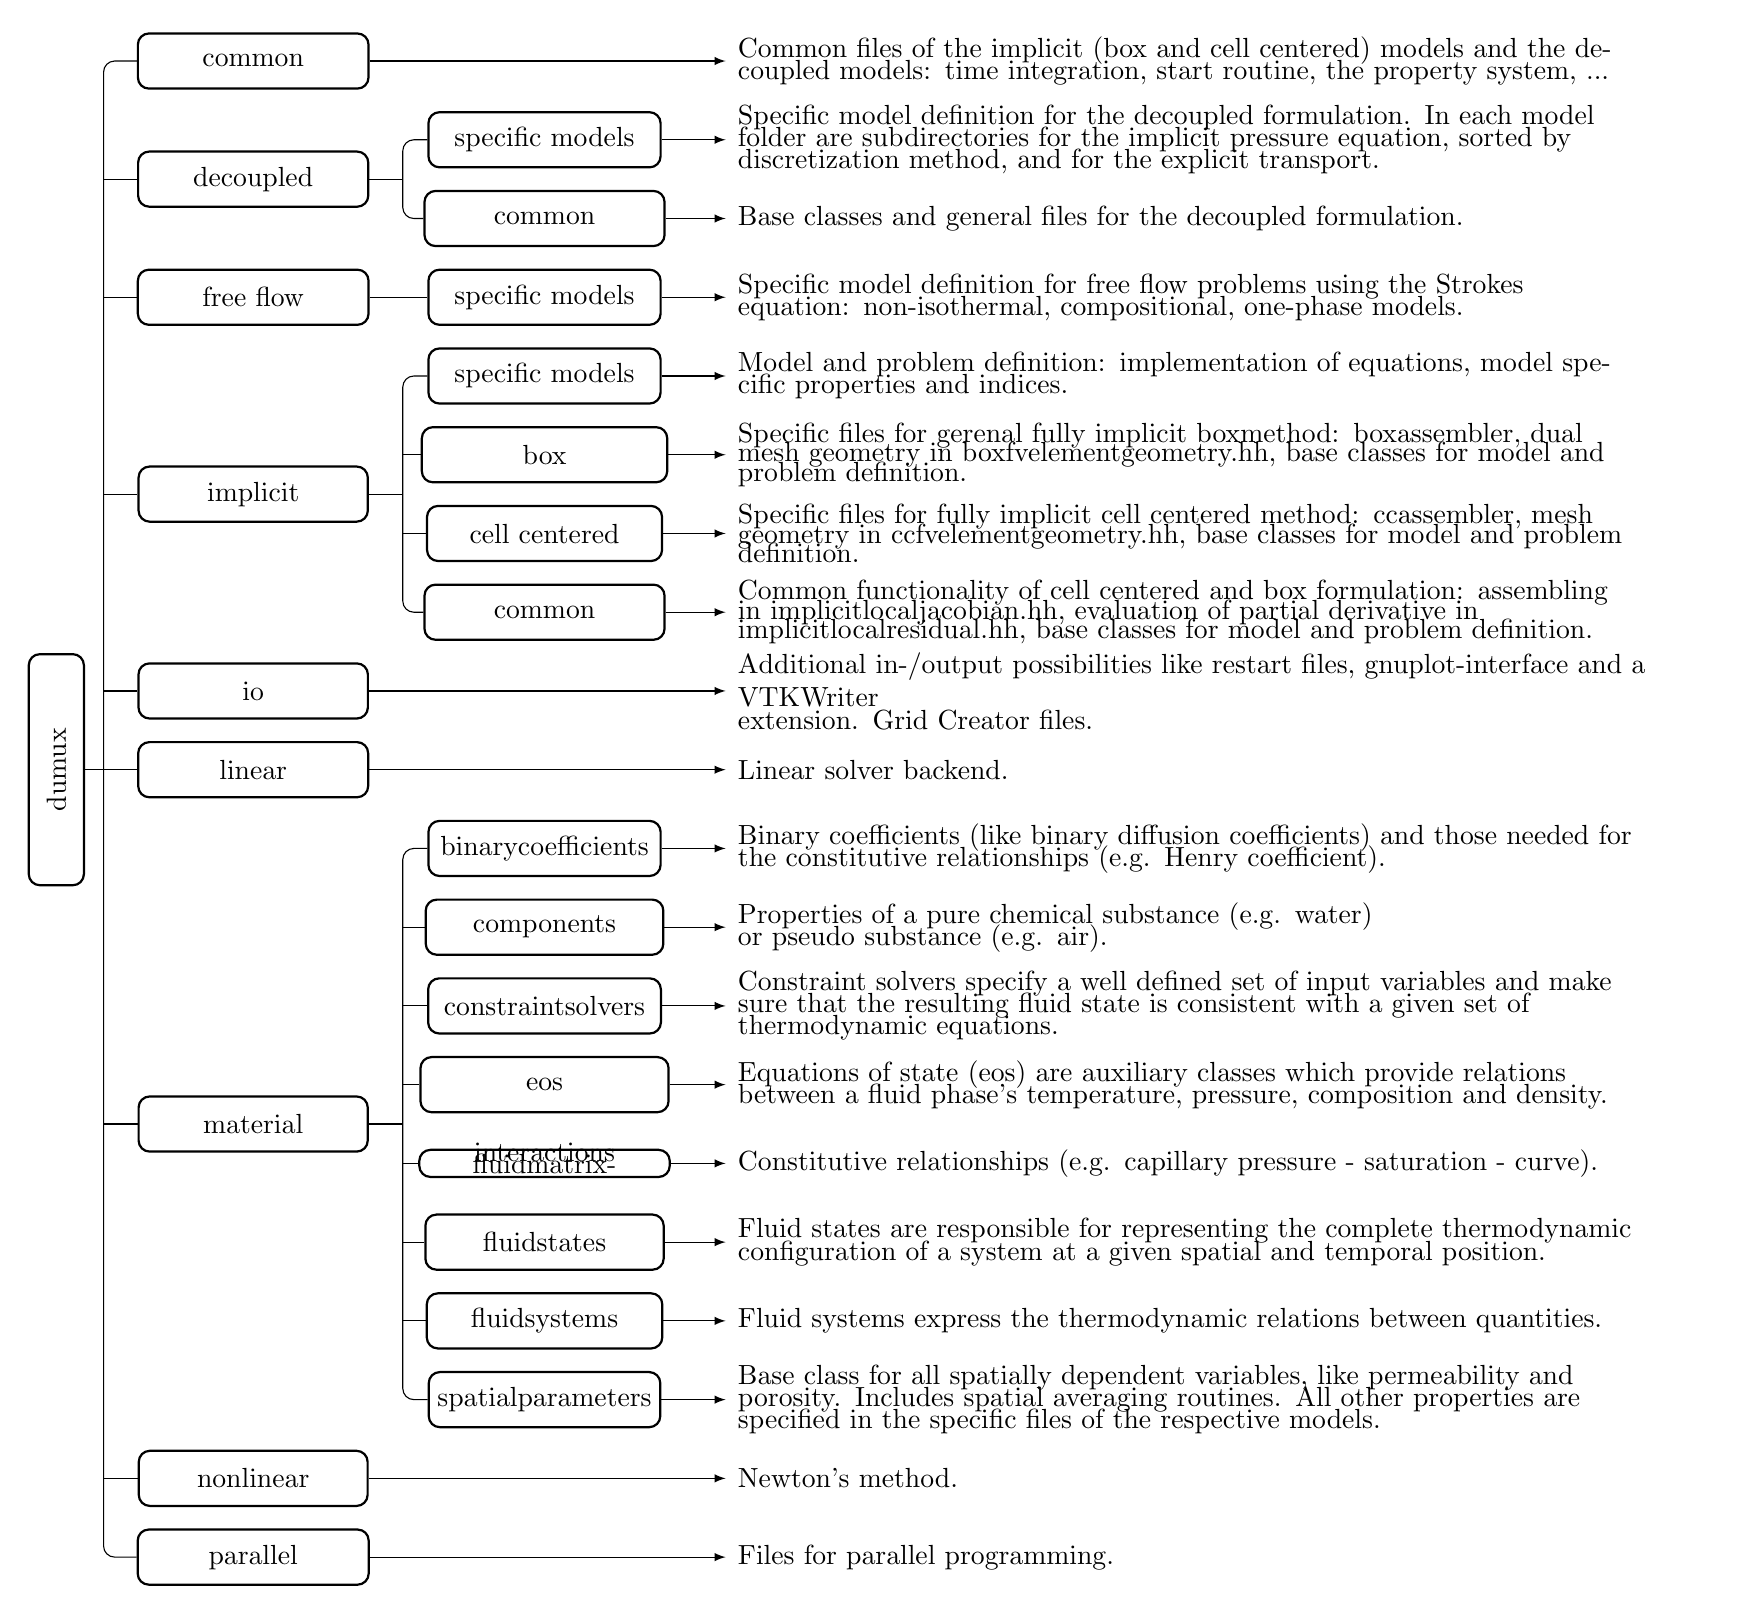
\begin{tikzpicture}[>=latex,inner xsep=0.15cm,rounded corners]
\node [minimum height=0.7cm,draw,inner xsep=0.94cm,rotate=90,thick] (d) at(-2,0) {dumux};
\node [minimum height=0.7cm,draw,inner xsep=1.03cm,thick] (lin) at(0.5,0) {linear};
\node [minimum height=0.7cm,draw,inner xsep=1.32cm,thick] (io) at(0.5,1) {io};

\node [minimum height=0.7cm,draw,inner xsep=0.87cm,thick] (imp) at(0.5,3.5) {implicit};
 \node [minimum height=0.7cm,draw,inner xsep=0.88cm,thick] (c1) at(4.2,2) {common};
 \node [minimum height=0.7cm,draw,inner xsep=0.54cm,thick] (cell) at(4.2,3) {cell centered};
 \node [minimum height=0.7cm,draw,inner xsep=1.28cm,thick] (box) at(4.2,4) {box};
 \node [minimum height=0.7cm,draw,inner xsep=0.33cm,thick] (spec1) at(4.2,5) {specific models};

\node [minimum height=0.7cm,draw,inner xsep=0.82cm,thick] (free) at(0.5,6) {free flow};
  \node [minimum height=0.7cm,draw,inner xsep=0.33cm,thick] (spec2) at(4.2,6) {specific models};

\node [minimum height=0.7cm,draw,inner xsep=0.7cm,thick] (dec) at(0.5,7.5) {decoupled};
 \node [minimum height=0.7cm,draw,inner xsep=0.88cm,thick] (c2) at(4.2,7) {common};
 \node [minimum height=0.7cm,draw,inner xsep=0.33cm,thick] (spec3) at(4.2,8) {specific models};

\node [minimum height=0.7cm,draw,inner xsep=0.82cm,thick] (c3) at(0.5,9) {common};

\node [minimum height=0.7cm,draw,inner xsep=0.82cm,thick] (m) at(0.5,-4.5) {material};
 \node [minimum height=0.7cm,draw,thick] (bin) at(4.2,-1) {binarycoefficients};
 \node [minimum height=0.7cm,draw,inner xsep=0.6cm,thick] (comp) at(4.2,-2) {components};
 \node [minimum height=0.7cm,draw,inner xsep=0.2cm,thick] (con) at(4.2,-3) {constraintsolvers};
 \node [minimum height=0.7cm,draw,inner xsep=1.34cm,thick] (eos) at(4.2,-4) {eos};
 \node [inner ysep=0.05cm,draw,text width=2cm,align=center,inner xsep=0.59cm,thick] (fi) at(4.2,-5) {fluidmatrix-\\[-16pt]interactions};
 \node [minimum height=0.7cm,draw,inner xsep=0.73cm,thick] (fstate) at(4.2,-6) {fluidstates};
 \node [minimum height=0.7cm,draw,inner xsep=0.56cm,thick] (fsys) at(4.2,-7) {fluidsystems};
 \node [minimum height=0.7cm,draw,inner xsep=0.11cm,thick] (s) at(4.2,-8) {spatialparameters};

\node [minimum height=0.7cm,draw,inner xsep=0.74cm,thick] (non) at(0.5,-9) {nonlinear};
\node [minimum height=0.7cm,draw,inner xsep=0.9cm,thick] (para) at(0.5,-10) {parallel};

\draw (d)--(lin);
\draw (-1.4,0)--(-1.4,9)--(c3);
\draw (-1.4,0)--(-1.4,-10)--(para);
\draw (-1.4,7.5)--(dec);
\draw (-1.4,6)--(free);
\draw (-1.4,3.5)--(imp);
\draw (-1.4,1)--(io);
\draw (-1.4,-4.5)--(m);
\draw (-1.4,-9)--(non);

\draw (dec)--(2.4,7.5);
\draw (spec3)--(2.4,8)--(2.4,7)--(c2);
\draw (free)--(spec2);
\draw (imp)--(2.4,3.5);
\draw (spec1)--(2.4,5)--(2.4,2)--(c1);
\draw (box)--(2.4,4);
\draw (cell)--(2.4,3);
\draw (m)--(2.4,-4.5);
\draw (bin)--(2.4,-1)--(2.4,-8)--(s);
\draw (comp)--(2.4,-2);
\draw (con)--(2.4,-3);
\draw (eos)--(2.4,-4);
\draw (fi)--(2.4,-5);
\draw (fstate)--(2.4,-6);
\draw (fsys)--(2.4,-7);

\draw [->](c3)--(6.5,9) node [right,text width=12.5cm,align=left]
  {Common files of the implicit (box and cell centered) models and the de-\\[-4pt]
   coupled models: time integration, start routine, the  property system, ...};
\draw [->](spec3)--(6.5,8) node [right,text width=12.5cm,align=left]
  {Specific model definition for the decoupled formulation. In each model \\[-4pt]
   folder are subdirectories for the implicit pressure  equation, sorted by \\[-4pt]discretization method, and for the explicit transport.};
\draw [->](c2)--(6.5,7) node [right,text width=12.5cm,align=left]
  {Base classes and general files for the decoupled formulation.};
\draw [->](spec2)--(6.5,6) node [right,text width=12.5cm,align=left]
  {Specific model definition for free flow problems using the Strokes \\[-4pt]
   equation: non-isothermal, compositional, one-phase models.};
\draw [->](spec1)--(6.5,5) node [right,text width=12.5cm,align=left]
  {Model and problem definition: implementation of equations, model spe-\\[-4pt]
   cific properties and indices.};
\draw [->](box)--(6.5,4) node [right,text width=12.5cm,align=left]
  {Specific files for gerenal fully implicit boxmethod: boxassembler, dual \\[-5pt]
   mesh geometry in boxfvelementgeometry.hh, base classes for model and \\[-5pt]problem definition.};
\draw [->](cell)--(6.5,3) node [right,text width=12.5cm,align=left]
  {Specific files for fully implicit cell centered method: ccassembler, mesh \\[-5pt]
   geometry in ccfvelementgeometry.hh, base classes for model and problem \\[-5pt]definition.};
\draw [->](c1)--(6.5,2) node [right,text width=12.5cm,align=left]
  {Common functionality of cell centered and box formulation: assembling \\[-5pt]
   in implicitlocaljacobian.hh, evaluation of partial derivative in \\[-5pt]implicitlocalresidual.hh, base classes for model and problem definition.};
\draw [->](io)--(6.5,1) node [right,text width=12.5cm,align=left]
  {Additional in-/output possibilities like restart files, gnuplot-interface and a VTKWriter \\[-4pt]
   extension. Grid Creator files.};
\draw [->](lin)--(6.5,0) node [right,text width=12.5cm,align=left] {Linear solver backend.};
\draw [->](bin)--(6.5,-1) node [right,text width=12.5cm,align=left]
  {Binary coefficients (like binary diffusion coefficients) and those needed for \\[-4pt]
   the constitutive relationships (e.g. Henry coefficient).};
\draw [->](comp)--(6.5,-2) node [right,text width=12.5cm,align=left]
  {Properties of a pure chemical substance (e.g. water) \\[-4pt]or pseudo substance (e.g. air).};
\draw [->](con)--(6.5,-3) node [right,text width=12.5cm,align=left]
  {Constraint solvers specify a well defined set of input variables and make \\[-4pt]
   sure that the resulting fluid state is consistent with a given set of \\[-4pt]thermodynamic equations.};
\draw [->](eos)--(6.5,-4) node [right,text width=12.5cm,align=left]
  {Equations of state (eos) are auxiliary classes which provide relations \\[-4pt]
   between a fluid phase's temperature, pressure, composition and density.};
\draw [->](fi)--(6.5,-5) node [right,text width=12.5cm,align=left]
  {Constitutive relationships (e.g. capillary pressure - saturation - curve).};
\draw [->](fstate)--(6.5,-6) node [right,text width=12.5cm,align=left]
  {Fluid states are responsible for representing the complete thermodynamic \\[-4pt]
   configuration of a system at a given spatial and temporal position.};
\draw [->](fsys)--(6.5,-7) node [right,text width=12.5cm,align=left]
  {Fluid systems express the thermodynamic relations between quantities.};
\draw [->](s)--(6.5,-8) node [right,text width=12.5cm,align=left]
  {Base class for all spatially dependent variables, like permeability and \\[-4pt]
   porosity. Includes spatial averaging routines. All other properties are \\[-4pt]
   specified in the specific files of the respective models.};
\draw [->](non)--(6.5,-9) node [right,text width=12.5cm,align=left]
  {Newton's method.};
\draw [->](para)--(6.5,-10) node [right,text width=12.5cm,align=left]
  {Files for parallel programming.};
\end{tikzpicture}
\caption{Structure of the directory \texttt{dumux} containing the \Dumux source files.
\todo[inline]{bei dieser Skizze sollten wir auch schauen ob die noch aktuell ist.}}
\label{fig:dumux-structure}
\end{sidewaysfigure}
